\documentclass[11pt,a4paper]{article}
\usepackage[margin=2.5cm]{geometry}
\usepackage{amsmath,amssymb,amsthm}
\usepackage{hyperref}
\usepackage{xcolor}
\usepackage{listings}
\usepackage{graphicx}
\usepackage{tikz}
\usetikzlibrary{arrows.meta,positioning,shapes,calc,decorations.pathreplacing}
\usepackage{booktabs}

\definecolor{colorInterval}{RGB}{68,221,255}
\definecolor{colorResult}{RGB}{255,136,68}
\definecolor{colorBase}{RGB}{255,221,68}
\definecolor{colorFill}{RGB}{255,68,170}
\definecolor{colorPartial}{RGB}{68,255,136}
\definecolor{colorEquiv}{RGB}{170,68,255}
\definecolor{codebg}{RGB}{24,24,36}
\definecolor{codetext}{RGB}{200,200,220}

\lstset{
  backgroundcolor=\color{codebg},
  basicstyle=\ttfamily\small\color{codetext},
  keywordstyle=\color{colorInterval},
  commentstyle=\color{gray},
  stringstyle=\color{colorPartial},
  breaklines=true,
  frame=single,
  rulecolor=\color{gray!40},
}

\hypersetup{colorlinks=true,linkcolor=blue,urlcolor=blue}

\title{\textbf{Univalence Walkthrough}\\
\large Detailed Technical Design for \texttt{cubical-viz}}
\author{Oguri Cap}
\date{March 2026}

\begin{document}
\maketitle
\tableofcontents
\newpage

%──────────────────────────────────────────────────────────────────────────────
\section{Goal and Scope}

This document is the implementation specification for the \textbf{Univalence
Walkthrough} feature of \texttt{cubical-viz}. It is a self-contained multi-stage
guided proof that shows how the Univalence principle is \emph{proved} (not
assumed) in cubical type theory using Glue types.

\medskip
\noindent\textbf{Target audience:} Students who have already explored the
Interval, Path Type, Transport, Kan Filling, and Glue Types pages.

\medskip
\noindent\textbf{Deliverable:}  A new sidebar entry ``Univalence'' under the
THEORY category, routing to a multi-stage interactive page.  Each of the four
stages is a full-height panel with a Three.js scene, a KaTeX proof fragment,
and a step panel.

%──────────────────────────────────────────────────────────────────────────────
\section{Mathematical Background}

\subsection{The Univalence Principle}

In homotopy type theory, the \emph{univalence axiom} asserts:
\[
  \mathrm{ua} : (A \simeq B) \to (A =_{\mathcal{U}} B)
\]
that equivalent types are equal.  In cubical type theory this is not an axiom
but a \emph{theorem}, proved by constructing a path in the universe $\mathcal{U}$
using \textbf{Glue types}.

\subsection{The Proof in One Paragraph}

Given an equivalence $e : A \simeq B$, we construct a line
$\mathrm{ua}(e) : \mathcal{U}$ parameterized by $i : \mathbb{I}$ as follows:
\[
  \mathrm{ua}(e)(i) \;=\;
  \mathrm{Glue}\bigl[\, i{=}0 \mapsto (A,\, e),\;\; i{=}1 \mapsto (B,\,\mathrm{id}_B) \,\bigr]\; B
\]
At $i=0$ this Glue type reduces definitionally to $A$; at $i=1$ it reduces to
$B$.  Hence $\mathrm{ua}(e)$ is a path $A =_{\mathcal{U}} B$.  Furthermore,
transport along this path computes as application of $e$:
$\mathrm{transp}^i\,(\mathrm{ua}(e)(i))\,a = e(a)$.

\subsection{Key Judgments Per Stage}

\begin{center}
\begin{tabular}{llp{7cm}}
\toprule
\textbf{Stage} & \textbf{Name} & \textbf{Key judgment} \\
\midrule
1 & Setup      & $\Gamma \vdash e : A \simeq B$ \\
2 & Glue line  & $\Gamma,\, i{:}\mathbb{I} \vdash
                  \mathrm{Glue}[\varphi \mapsto (T,f)]\,B : \mathcal{U}$ \\
3 & Path in $\mathcal{U}$ &
                  $\Gamma \vdash \mathrm{ua}(e) : A =_{\mathcal{U}} B$ \\
4 & Transport  & $\Gamma \vdash \mathrm{transp}^i(\mathrm{ua}(e)(i))\,a
                  \equiv e(a) : B$ \\
\bottomrule
\end{tabular}
\end{center}

%──────────────────────────────────────────────────────────────────────────────
\section{Page Architecture}

\subsection{Route and Component Tree}

\begin{lstlisting}[language=]
App.svelte
  {:else if current === 'univalence'}
    <Univalence />          // top-level orchestrator

Univalence.svelte
  <StageNav />              // progress bar / stage tabs
  {#if stage === 0} <UniSetup />
  {#if stage === 1} <UniGlue />
  {#if stage === 2} <UniPath />
  {#if stage === 3} <UniTransport />

Each stage component (e.g. UniSetup.svelte):
  <Rule rule={stageRule} />    // reuses Rule.svelte wrapper
\end{lstlisting}

\subsection{StageNav Component}

A horizontal progress bar above the content area:

\begin{center}
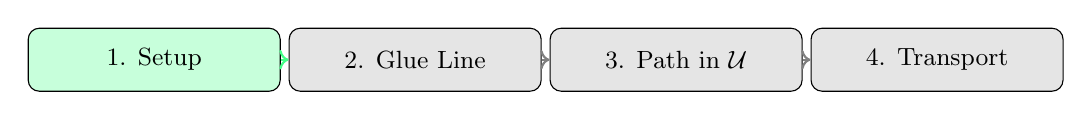
\begin{tikzpicture}[node distance=0cm]
  \node[draw,rounded corners,fill=colorPartial!30,minimum width=3.2cm,minimum height=0.8cm,align=center,font=\small] (s1) {1. Setup};
  \node[draw,rounded corners,fill=gray!20,minimum width=3.2cm,minimum height=0.8cm,align=center,font=\small,right=0.1cm of s1] (s2) {2. Glue Line};
  \node[draw,rounded corners,fill=gray!20,minimum width=3.2cm,minimum height=0.8cm,align=center,font=\small,right=0.1cm of s2] (s3) {3. Path in $\mathcal{U}$};
  \node[draw,rounded corners,fill=gray!20,minimum width=3.2cm,minimum height=0.8cm,align=center,font=\small,right=0.1cm of s3] (s4) {4. Transport};
  \draw[->,thick,colorPartial] (s1.east) -- (s2.west);
  \draw[->,thick,gray] (s2.east) -- (s3.west);
  \draw[->,thick,gray] (s3.east) -- (s4.west);
\end{tikzpicture}
\end{center}

\noindent The active stage is highlighted in \textcolor{colorPartial}{green}.
Completed stages are \textcolor{colorInterval}{cyan}. Future stages are gray.
Clicking a completed stage navigates back.

A ``Continue →'' button at the bottom-right of the step panel advances to the
next stage (enabled only when the user reaches the last step of the current stage).

\subsection{State Management}

\begin{lstlisting}[language=javascript]
// in Univalence.svelte
let stage = $state(0);           // 0-3
let stageCompleted = $state([false, false, false, false]);

function advanceStage() {
  stageCompleted[stage] = true;
  stage = Math.min(stage + 1, 3);
}
\end{lstlisting}

%──────────────────────────────────────────────────────────────────────────────
\section{Stage 1: Setup}

\subsection{Concept}

Introduce the two types $A$ and $B$ and the equivalence $e : A \simeq B$.
Recall that an equivalence is a function $f : A \to B$ with a contractible
fiber — equivalently, a homotopy equivalence.

\subsection{KaTeX Judgment}

\[
  \frac{
    \Gamma \vdash A : \mathcal{U}
    \qquad
    \Gamma \vdash B : \mathcal{U}
    \qquad
    \Gamma \vdash e : A \simeq B
  }{
    \Gamma \vdash \mathrm{ua}(e) : A =_{\mathcal{U}} B
  }\ (\text{ua})
\]

\subsection{3D Scene}

\begin{itemize}
  \item Two large spheres (radius 0.9):
    \begin{itemize}
      \item $A$ at $(-3, 0, 0)$, color \textcolor{colorInterval}{\texttt{INTERVAL}} (0x44DDFF).
      \item $B$ at $(+3, 0, 0)$, color \textcolor{colorResult}{\texttt{RESULT}} (0xFF8844).
    \end{itemize}
  \item A \textbf{curved arrow} from $A$ to $B$ using a
    \texttt{QuadraticBezierCurve3} with control point $(0, 2, 1)$:
    gradient \textcolor{colorInterval}{cyan} $\to$ \textcolor{colorResult}{orange},
    with an animated arrowhead traveling along the curve.
  \item Label sprites: ``$A$'' above the left sphere, ``$B$'' above the right
    sphere, ``$e$'' midway on the arc.
  \item A faint dotted horizontal line segment between $A$ and $B$
    (dim white, opacity 0.2), labeled ``$i \in [0,1]$'' — hinting at the path
    to be constructed.
  \item Camera: $(0, 1, 9)$ looking at $(0, 0, 0)$.
\end{itemize}

\subsection{Steps}

\begin{enumerate}
  \item \textbf{Two types} — ``$A$ and $B$ are types in the universe $\mathcal{U}$.
    In the univalence proof, we start with an equivalence $e : A \simeq B$.''
    \textit{(timeRange: [0, 0.4])}
  \item \textbf{Equivalence} — ``An equivalence $e : A \simeq B$ is a function
    $f : A \to B$ with homotopy inverse. It witnesses that $A$ and $B$ have the
    same structure.''
    \textit{(timeRange: [0.4, 0.7])}
  \item \textbf{Goal} — ``We want to produce a \emph{path} $\mathrm{ua}(e) : A
    =_{\mathcal{U}} B$ — an element of the identity type in the universe. This
    path does not exist in MLTT without an axiom; in cubical TT we construct it.''
    \textit{(timeRange: [0.7, 1.0])}
\end{enumerate}

\subsection{Term Mappings}
\begin{center}
\begin{tabular}{ll}
\toprule \textbf{termKey} & \textbf{3D object} \\\midrule
\texttt{A} & Left sphere \\ \texttt{B} & Right sphere \\
\texttt{e} & Arc line \\ \bottomrule
\end{tabular}
\end{center}

%──────────────────────────────────────────────────────────────────────────────
\section{Stage 2: Glue Line}

\subsection{Concept}

Construct the Glue type indexed by $i : \mathbb{I}$.  At each $i$, the type is
$\mathrm{Glue}[\,i{=}0\mapsto(A,e),\;i{=}1\mapsto(B,\mathrm{id})\,]\,B$.
This is a \emph{line of types} in $\mathcal{U}$.

\subsection{KaTeX Judgment}

\[
  \Gamma,\,i{:}\mathbb{I} \;\vdash\;
  \underbrace{
    \mathrm{Glue}\bigl[\,i{=}0\mapsto(A,e),\;\;i{=}1\mapsto(B,\mathrm{id})\,\bigr]\,B
  }_{\mathrm{ua}(e)(i)} : \mathcal{U}
\]

\subsection{3D Scene}

The scene transitions from Stage~1's two-sphere layout into a \textbf{cylinder}
connecting $A$ to $B$.

\begin{itemize}
  \item The curved arc from Stage~1 thickens into a \texttt{CylinderGeometry}
    (radiusTop 0.25, radiusBottom 0.25, height 6) between $(-3,0,0)$ and
    $(3,0,0)$, oriented along the X-axis.
    Color: gradient texture from \textcolor{colorInterval}{cyan} (left) to
    \textcolor{colorResult}{orange} (right).
    In Three.js, simulate the gradient by two
    \texttt{MeshBasicMaterial} half-cylinders, or use vertex colors on a
    \texttt{TubeGeometry} following the path.
  \item A thin \textbf{slider sphere} (radius 0.18, color white) moves along
    the cylinder at $x = \mathrm{lerp}(-3, 3, t)$, representing the current
    value of $i$.
  \item \textbf{End cap labels}: ``$\mathrm{Glue}(0) \equiv A$'' at the left
    end; ``$\mathrm{Glue}(1) \equiv B$'' at the right end.
  \item \textbf{Cross-section indicator}: At the slider position, draw a thin
    circle (torus, radius 0.28, tube 0.02) perpendicular to the cylinder axis,
    color \textcolor{colorFill}{\texttt{FILL\_RESULT}} (0xFF44AA). A text sprite
    above it reads ``$\mathrm{Glue}(i)$''.
  \item The two original spheres ($A$ and $B$) remain visible at the ends,
    slightly smaller (radius 0.7).
  \item Camera: $(0, 2, 9)$ looking at $(0, 0, 0)$.
\end{itemize}

\subsection{Steps}

\begin{enumerate}
  \item \textbf{Glue type} — ``A Glue type bundles a base type $B$ with partial
    data specifying how certain faces map to other types via equivalences.
    Here, the face $i{=}0$ is glued to $A$ via $e$.''
    \textit{(timeRange: [0, 0.35])}
  \item \textbf{Line of types} — ``For each $i : \mathbb{I}$, the Glue type gives
    a type $\mathrm{ua}(e)(i)$.  The slider shows $i$ varying: at the left end
    the type is definitionally $A$, at the right it is $B$.''
    \textit{(timeRange: [0.35, 0.7])}
  \item \textbf{Boundary conditions} — ``The definitional equalities
    $\mathrm{Glue}(0) \equiv A$ and $\mathrm{Glue}(1) \equiv B$ are enforced by
    the Glue type former's reduction rules — no propositional proof required.''
    \textit{(timeRange: [0.7, 1.0])}
\end{enumerate}

\subsection{Term Mappings}
\begin{center}
\begin{tabular}{ll}
\toprule \textbf{termKey} & \textbf{3D object} \\\midrule
\texttt{glue\_line} & Cylinder/tube mesh \\
\texttt{A\_end} & Left sphere \\
\texttt{B\_end} & Right sphere \\
\texttt{glue\_i} & Slider sphere + torus cross-section \\
\bottomrule
\end{tabular}
\end{center}

%──────────────────────────────────────────────────────────────────────────────
\section{Stage 3: Path in the Universe}

\subsection{Concept}

The line of Glue types \emph{is} a path in $\mathcal{U}$.  Show the universe as
an ambient space and display the path $\mathrm{ua}(e)$ living inside it.

\subsection{KaTeX Judgment}

\[
  \Gamma \;\vdash\; \lambda\,i.\;\mathrm{Glue}[\cdots]\,B \;:\; A =_{\mathcal{U}} B
\]

\subsection{3D Scene}

\begin{itemize}
  \item \textbf{Universe plane}: a large \texttt{GridHelper} at $y = -2.5$,
    size 20, divisions 20, colors \texttt{0x222244}/\texttt{0x333366}.  This
    represents $\mathcal{U}$ as an ambient ``ground plane''.
  \item \textbf{Path curve}: the cylinder from Stage~2 is re-rendered as a
    thinner curved line (the path $\mathrm{ua}(e)$), floating above the
    universe plane.  Use a \texttt{QuadraticBezierCurve3} from $(-3, 0, 0)$ to
    $(3, 0, 0)$ with control point $(0, 1.5, 1.5)$, gradient
    \textcolor{colorInterval}{cyan}$\to$\textcolor{colorResult}{orange}.
  \item \textbf{Type labels}: Small floating text boxes labeled ``$A$'' and
    ``$B$'' at the two ends, connected to the path endpoints by thin vertical
    lines to the grid below.
  \item \textbf{Path label}: ``$\mathrm{ua}(e)$'' as a text sprite above the
    midpoint of the arc.
  \item \textbf{Camera}: zoomed out to $(0, 4, 14)$ looking at $(0, 0, 0)$,
    giving a panoramic view of the ``universe''.
\end{itemize}

\subsection{Camera Transition}

When Stage~3 mounts, animate the camera from its Stage~2 position
$(0, 2, 9)$ to $(0, 4, 14)$ over 1.5 seconds using a \texttt{TWEEN}-style
lerp:
\begin{lstlisting}[language=javascript]
// In onMount / setup:
const startPos = new THREE.Vector3(0, 2, 9);
const endPos   = new THREE.Vector3(0, 4, 14);
// lerp over elapsed 0..1.5s during first 1.5s of animation
\end{lstlisting}

\subsection{Steps}

\begin{enumerate}
  \item \textbf{The universe $\mathcal{U}$} — ``The universe $\mathcal{U}$
    contains all types as points. A path in $\mathcal{U}$ between $A$ and $B$
    is exactly an element of $A =_{\mathcal{U}} B$.''
    \textit{(timeRange: [0, 0.4])}
  \item \textbf{ua(e) as a path} — ``The line of Glue types $i \mapsto
    \mathrm{Glue}[\cdots]B$ is a \emph{term} of type $A =_{\mathcal{U}} B$.
    It is a literal path in the universe from $A$ to $B$.''
    \textit{(timeRange: [0.4, 0.75])}
  \item \textbf{Univalence achieved} — ``This is the univalence map:
    $\mathrm{ua} : (A \simeq B) \to (A =_{\mathcal{U}} B)$.  No axiom was
    needed — the path was constructed from the Glue type former.''
    \textit{(timeRange: [0.75, 1.0])}
\end{enumerate}

%──────────────────────────────────────────────────────────────────────────────
\section{Stage 4: Transport}

\subsection{Concept}

Verify that transporting along $\mathrm{ua}(e)$ computes as application of $e$.
This is the \emph{computation rule} for univalence:
$\mathrm{transp}^i\,(\mathrm{ua}(e)(i))\,a \equiv e(a)$.

\subsection{KaTeX Judgment}

\[
  \Gamma \;\vdash\; \mathrm{transp}^i\bigl(\mathrm{ua}(e)(i)\bigr)\,a
  \;\equiv\; e(a) \;:\; B
\]

\subsection{3D Scene}

A split composition: the left half shows the path $\mathrm{ua}(e)$ (from
Stage~3, simplified); the right half shows the transport computation.

\begin{itemize}
  \item \textbf{Left panel} (world $x < 0$, i.e.\ the path in $\mathcal{U}$):
    \begin{itemize}
      \item Small versions of $A$ (cyan sphere, radius 0.5, at $(-3, 0, 0)$)
        and $B$ (orange sphere, radius 0.5, at $(-0.5, 0, 0)$).
      \item The path arc between them (gradient, thin).
      \item A moving point on the arc, colored white.
    \end{itemize}
  \item \textbf{Right panel} (world $x > 0$, i.e.\ the fiber):
    \begin{itemize}
      \item A small cyan sphere labeled ``$a : A$'' at $(1, 0, 0)$.
      \item An animated \textbf{morphing dot}: starts at $(1, 0, 0)$ (position
        in $A$, cyan) and travels along a Bézier arc to $(3.5, 0, 0)$ (position
        in $B$, orange), driven by the same $t$ as the path traversal.
      \item Label: ``$e(a)$'' appears at the orange end as the dot arrives.
      \item A thin vertical \textbf{separator line} at $x = 0$ from $y=-2$ to
        $y=2$, color dim white.
    \end{itemize}
  \item Camera: $(0, 2, 10)$ looking at $(0, 0, 0)$.
\end{itemize}

\subsection{Steps}

\begin{enumerate}
  \item \textbf{Recall transport} — ``Transport along a path $p : A =_{\mathcal{U}}
    B$ sends elements of $A$ to elements of $B$: $\mathrm{transp}^i\,p(i)\,a : B$.''
    \textit{(timeRange: [0, 0.35])}
  \item \textbf{Transport along ua(e)} — ``Transporting $a : A$ along
    $\mathrm{ua}(e)$ moves $a$ from the fiber at $i=0$ (type $A$) to the fiber
    at $i=1$ (type $B$).''
    \textit{(timeRange: [0.35, 0.7])}
  \item \textbf{Computation rule} — ``By the definitional reduction of Glue
    types, this transport \emph{computes} to $e(a)$: the underlying function of
    the equivalence.  This is the \emph{transport computation rule} for
    univalence.''
    \textit{(timeRange: [0.7, 1.0])}
\end{enumerate}

\subsection{Completion}

After reaching the final step of Stage~4, a \textbf{completion overlay}
appears:

\begin{itemize}
  \item Semi-transparent dark backdrop over the 3D scene.
  \item Centered panel:
    \begin{itemize}
      \item Header: ``Univalence Proved! 🎉''
      \item Summary: the full chain
        $e \mapsto \mathrm{ua}(e) \mapsto \mathrm{transp}^i(\mathrm{ua}(e)(i))
        \equiv e$ displayed in KaTeX.
      \item Two buttons: ``Review from Stage 1'' (resets stage to 0) and
        ``Explore related rules'' (links to Glue Types and Transport pages).
    \end{itemize}
\end{itemize}

%──────────────────────────────────────────────────────────────────────────────
\section{Component Specifications}

\subsection{Univalence.svelte}

\begin{lstlisting}[language=html]
<script lang="ts">
  import StageNav from './univalence/StageNav.svelte';
  import UniSetup from './univalence/UniSetup.svelte';
  import UniGlue from './univalence/UniGlue.svelte';
  import UniPath from './univalence/UniPath.svelte';
  import UniTransport from './univalence/UniTransport.svelte';

  let stage = $state(0);
  let completed = $state([false,false,false,false]);

  function advance() {
    completed[stage] = true;
    if (stage < 3) stage++;
  }
</script>

<div class="univalence-page">
  <StageNav {stage} {completed} onSelect={(s) => stage = s} />
  <div class="stage-content">
    {#if stage === 0}<UniSetup onComplete={advance} />{/if}
    {#if stage === 1}<UniGlue onComplete={advance} />{/if}
    {#if stage === 2}<UniPath onComplete={advance} />{/if}
    {#if stage === 3}<UniTransport onComplete={advance} />{/if}
  </div>
</div>
\end{lstlisting}

\subsection{StageNav.svelte}

Props: \texttt{stage: number}, \texttt{completed: boolean[]},
\texttt{onSelect: (n: number) => void}.

Renders four buttons.  A button for stage $k$ is:
\begin{itemize}
  \item \textit{Active} (\texttt{stage === k}): green background.
  \item \textit{Completed} (\texttt{completed[k]}): cyan background, clickable.
  \item \textit{Future}: gray, disabled.
\end{itemize}

\subsection{UniSetup / UniGlue / UniPath / UniTransport}

Each wraps a \texttt{RuleDefinition} (same interface as all other rules) and
passes it to \texttt{Rule.svelte}. Additionally each accepts an
\texttt{onComplete: () => void} callback, which it forwards to the ``Continue
→'' button that replaces the usual ``Next →'' at the final step.

The \texttt{RuleDefinition} for each stage:
\begin{lstlisting}[language=typescript]
const stageRule: RuleDefinition = {
  id:          'univalence-setup',       // unique id
  name:        'Setup',
  katex:       '...',                    // judgment string
  description: '...',
  setup:       (scene, camera) => { ... },
  update:      (t, elapsed) => { ... },
  cleanup:     (scene) => { ... },
  steps:       [ ... ],                  // 3 steps per stage
  termMappings: { ... },
};
\end{lstlisting}

\subsection{Completion Overlay}

Implemented inside \texttt{UniTransport.svelte}. Triggered when the user
reaches step 3 and the animation completes one cycle:

\begin{lstlisting}[language=html]
{#if showCompletion}
  <div class="completion-overlay">
    <div class="completion-panel">
      <h2>Univalence Proved! 🎉</h2>
      <!-- KaTeX summary -->
      <div class="summary">{@html katexSummary}</div>
      <button onclick={() => stage = 0}>Review from Stage 1</button>
      <button onclick={() => navigate('glue-type-rule')}>
        Explore: Glue Types
      </button>
    </div>
  </div>
{/if}
\end{lstlisting}

%──────────────────────────────────────────────────────────────────────────────
\section{File Structure}

\begin{lstlisting}[language=]
src/lib/
  univalence/
    Univalence.svelte        # orchestrator
    StageNav.svelte          # progress bar
    UniSetup.svelte          # stage 1
    UniGlue.svelte           # stage 2
    UniPath.svelte           # stage 3
    UniTransport.svelte      # stage 4

src/lib/types.ts             # add 'univalence' to VisualizationType,
                             # add to THEORY category
src/App.svelte               # add render branch (isStandalone)
\end{lstlisting}

%──────────────────────────────────────────────────────────────────────────────
\section{Implementation Order for Copilot}

This is a large task that should be split into two Copilot sessions to stay
within context limits.

\paragraph{Session A — Scaffolding + Stages 1 \& 2.}
\begin{enumerate}
  \item Create \texttt{src/lib/univalence/} directory.
  \item Implement \texttt{StageNav.svelte}.
  \item Implement \texttt{Univalence.svelte} orchestrator with empty stage stubs.
  \item Register \texttt{'univalence'} in \texttt{types.ts} and \texttt{App.svelte}.
  \item Implement \texttt{UniSetup.svelte} (Stage~1: two spheres, arc, 3 steps).
  \item Implement \texttt{UniGlue.svelte} (Stage~2: cylinder, slider, 3 steps).
  \item Build passes. Commit: ``Univalence: scaffold + stages 1-2''.
\end{enumerate}

\paragraph{Session B — Stages 3, 4 \& Completion.}
\begin{enumerate}
  \item Implement \texttt{UniPath.svelte} (Stage~3: universe grid, zoomed-out path).
  \item Implement \texttt{UniTransport.svelte} (Stage~4: split scene, morphing dot).
  \item Add completion overlay to \texttt{UniTransport.svelte}.
  \item Final build pass and commit: ``Univalence: stages 3-4 + completion overlay''.
\end{enumerate}

%──────────────────────────────────────────────────────────────────────────────
\section{Color Summary}

\begin{center}
\begin{tabular}{lll}
\toprule
\textbf{Concept} & \textbf{Constant} & \textbf{Hex} \\\midrule
Type $A$ & \texttt{INTERVAL} & \texttt{0x44DDFF} \\
Type $B$ & \texttt{RESULT}   & \texttt{0xFF8844} \\
Equivalence $e$ & gradient INTERVAL→RESULT & --- \\
Glue line / path ua(e) & gradient INTERVAL→RESULT & --- \\
Cross-section $\mathrm{Glue}(i)$ & \texttt{FILL\_RESULT} & \texttt{0xFF44AA} \\
Universe grid & \texttt{0x222244}/\texttt{0x333366} & --- \\
Transport dot start & \texttt{INTERVAL} & \texttt{0x44DDFF} \\
Transport dot end & \texttt{RESULT} & \texttt{0xFF8844} \\
Stage: active & \texttt{PARTIAL\_DATA} & \texttt{0x44FF88} \\
Stage: completed & \texttt{INTERVAL} & \texttt{0x44DDFF} \\
Stage: future & gray & \texttt{0x555566} \\
\bottomrule
\end{tabular}
\end{center}

%──────────────────────────────────────────────────────────────────────────────
\section{Risks and Mitigations}

\begin{center}
\begin{tabular}{p{5cm}p{4cm}p{4cm}}
\toprule
\textbf{Risk} & \textbf{Likelihood} & \textbf{Mitigation} \\\midrule
Copilot generates incorrect Three.js for cylinder gradient &
Medium &
Use two half-cylinders with solid colors (INTERVAL / RESULT) instead of a
gradient material \\
\addlinespace
Camera transition causes jank when switching stages &
Low &
Skip camera animation in first version; set camera directly in \texttt{setup()} \\
\addlinespace
Completion overlay KaTeX string too long &
Low &
Use \texttt{displayMode: true} and wrap in a scrollable div \\
\addlinespace
\texttt{Rule.svelte} doesn't pass \texttt{onComplete} through &
Medium &
Pass it as a prop to the \texttt{StepPanel}; or handle in each stage component
by watching \texttt{activeStep === rule.steps.length - 1} \\
\bottomrule
\end{tabular}
\end{center}

\end{document}
